%TCIDATA{Version=5.50.0.2890}
%TCIDATA{LaTeXparent=0,0,NoticeDKE.tex}
                      

\section{Electron Dynamics in an Axisymmetric Torus\label{dynamics}}

In this section, we first introduce the axisymmetric toroidal magnetic
equilibrium applicable to tokamaks and STs. The particle motion in this
magnetic field is described and the drift across magnetic flux surfaces is
calculated. In addition, the bounce-averaging operation is defined in the
zero-banana width limit, when the drifts can be neglected in first
approximation. The results presented here are not derived from first
principles, although this has been done in previous works refered to in this
section. The properties of the equilibrium magnetic field are obtained from
ideal MHD equations \cite{fre87b1} \cite{haz91b1}. The motion of particles
in a non-uniform magnetic field has been derived by expanding the equation
of motion to orders of $\rho_{L}/L_{B}\ll1$ where $\rho_{L}$ is the Larmor
radius and $L_{B}$ is the scale length of magnetic field variations \cite%
{nor63b1} \cite{nor78}. Equivalently, these equation have been derived using
an Hamiltonian approach \cite{lit81}.

\subsection{Toroidal plasma field geometry and configuration space
coordinates systems\label{torgeom}}

\begin{figure}[tbh]
\begin{center}
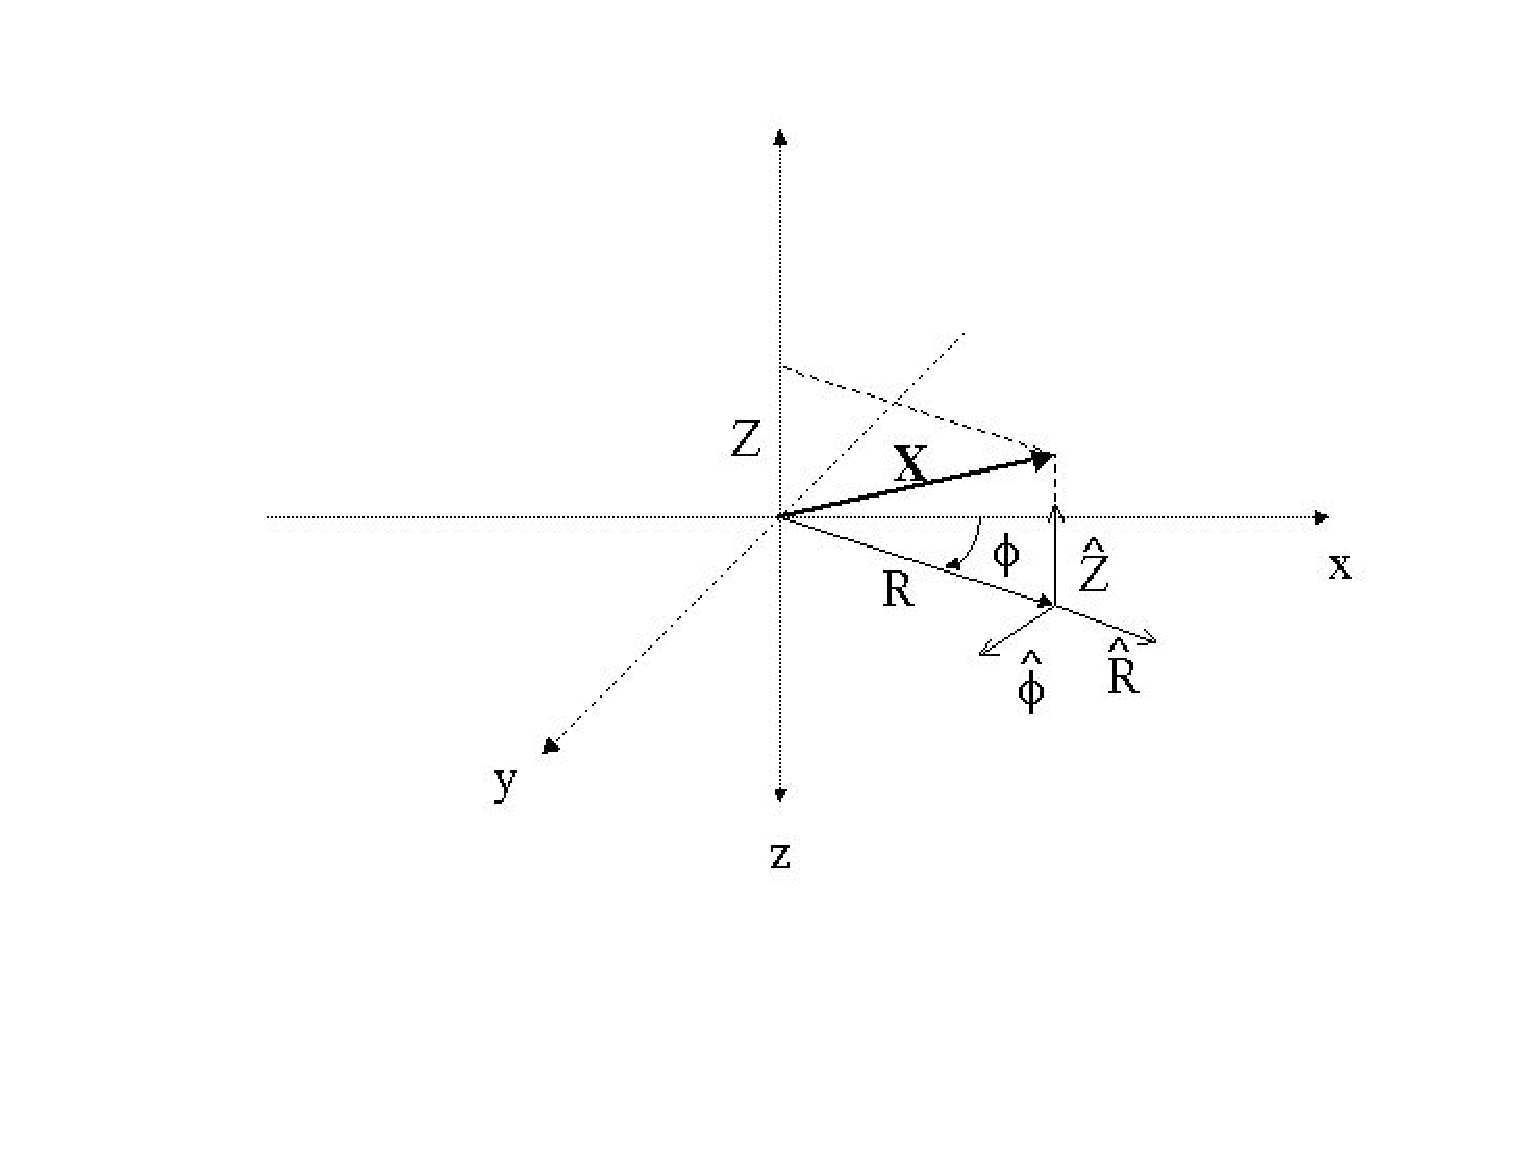
\includegraphics[width=3.6in]{figures/RZphi.eps}
\end{center}
\caption{Cylindrical coordinate system $\left( R,Z,\protect\phi\right) $ for
axisymmetric toroidal plasmas.}
\label{figRZphi}
\end{figure}

A natural coordinates system for an axisymmetric toroidal plasma is the
cylindrical system $\left( R,Z,\phi\right) $, defined in (\ref{RZphidef})
and shown in Fig. \ref{figRZphi}, where $R$ is the distance from the torus
axis of symmetry, $Z$ is the (generally vertical) position along this axis,
and $\phi$ is the angle in the toroidal direction. The system $\left(
R,Z,\phi\right) $ is oriented such that the toroidal magnetic field be
positive $\mathbf{B}\cdot\mathbf{\nabla}\phi>0$. In other words, if the
toroidal field is directed clockwise from a top view, then $\mathbf{\nabla}Z$
is oriented towards the top of the torus. Otherwise, it is oriented towards
the bottom of the torus. The corresponding local direct orthonormal vector
basis is $\left( \widehat{\mathbf{R}},\widehat{\mathbf{Z}},\widehat {\mathbf{%
\phi}}\right) $, defined in (\ref{RZphibasis}), with (\ref{contRZphi})%
\begin{equation}
\begin{array}{l}
\widehat{\mathbf{R}}=\mathbf{\nabla}R \\ 
\widehat{\mathbf{Z}}=\mathbf{\nabla}Z \\ 
\widehat{\mathbf{\phi}}=R\mathbf{\nabla}\phi%
\end{array}
\label{RZphi}
\end{equation}
Many useful geometrical and differential properties of this system are
derived in Appendix \ref{curvilinear}. Note that with our definitions, the
angle $\phi$ is oriented in the opposite direction from the one used
generally in ideal MHD, where the direct orthonormal vector basis is $\left( 
\widehat{\mathbf{R}},\widehat{\mathbf{\phi}},\widehat{\mathbf{Z}}\right) $.
The present prescription allows us to use the same toroidal coordinate $\phi$
throughout various coordinate systems defined below.

In a toroidal axisymmetric geometry, the equilibrium magnetic field can be
expressed generally as \cite{haz91b1} 
\begin{equation}
\mathbf{B}=I\left( \psi\right) \mathbf{\nabla}\phi+\mathbf{\nabla}\phi \times%
\mathbf{\nabla}\psi   \label{B}
\end{equation}
where $\psi$ is called the \textit{magnetic flux function} and $I\left(
\psi\right) $ is a free function related to the toroidal magnetic field, and
which accounts for the plasma dia- or paramagnetism. In an axisymmetric
system, $\psi$ is independent of $\phi$ and therefore $\mathbf{\nabla}%
\psi\cdot\mathbf{\nabla}\phi=0$ and we get from (\ref{B}) that $\mathbf{B}%
\cdot\mathbf{\nabla}\psi=0$. The magnetic field is therefore included in
nested surfaces of constant $\psi$, called \textit{flux surfaces}.

\begin{figure}[tbh]
\begin{center}
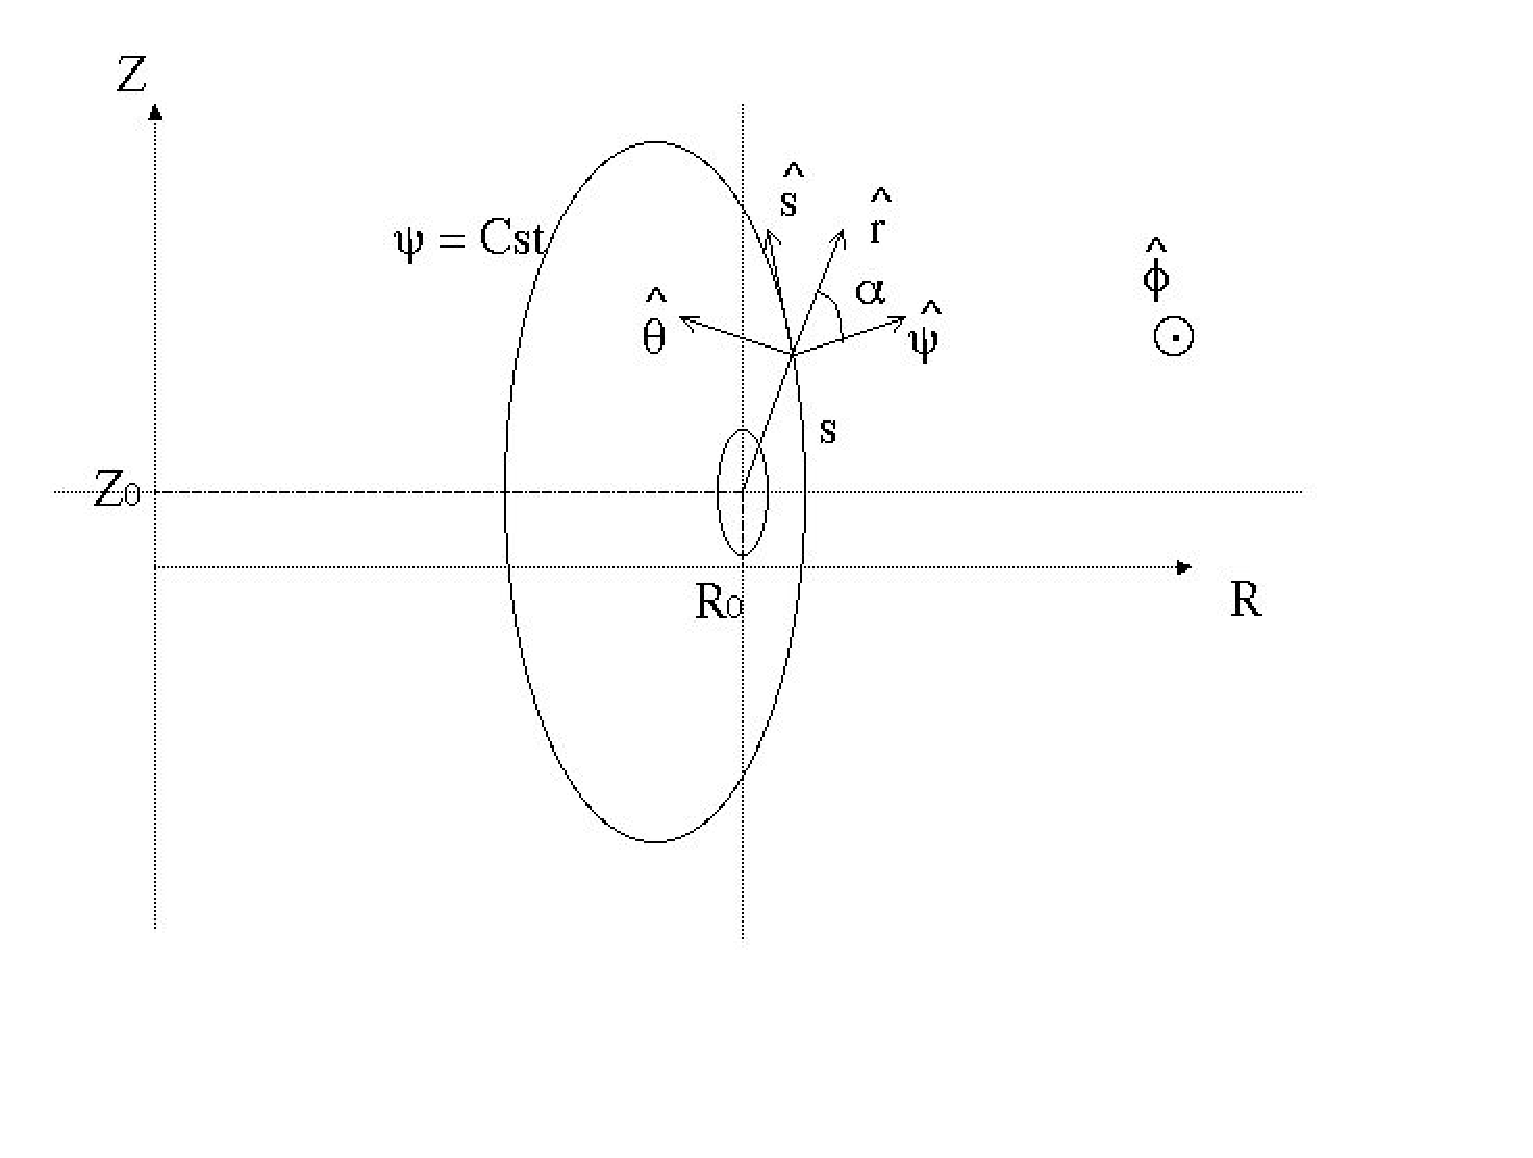
\includegraphics[width=3.6in]{figures/psisphi.eps}
\end{center}
\caption{Flux coordinates system $\left( \protect\psi,s,\protect\phi\right) $
for axisymmetric toroidal plasmas with closed nested flux-surfaces.}
\label{figpsisphi}
\end{figure}

A consequence of the axisymmetric magnetic equilibrium is the existence of a
magnetic axis in the toroidal direction, located at the fixed position $%
\left( R_{p},Z_{p}\right) ,$which corresponds to the innermost flux-surface.
The magnetic axis is an extremum of the magnetic flux function $\psi$. The
value of $\psi$ on axis can be arbitrarily chosen as $\psi=0$. Using this
axis as a reference, we define the coordinate system $\left(
\psi,s,\phi\right) $, shown in Fig. \ref{figpsisphi}, where the distance $s$
is the curvilinear length along the poloidal magnetic field lines (\ref%
{psisphidef}). In this study, we assume that the magnetic field amplitude
has only one maximum and one minimum on the flux-surface, which is generally
the case for tokamaks and STs%
\begin{equation}
\begin{array}{l}
B_{\max}\left( \psi\right) \equiv\max\limits_{s}\left\{ B\left(
\psi,s\right) \right\} \\ 
B_{0}\left( \psi\right) \equiv\min\limits_{s}\left\{ B\left( \psi,s\right)
\right\}%
\end{array}%
\end{equation}
and we choose the origin of $s$ to be at the position of minimum $B$-field
amplitude within a flux-surface. 
\begin{equation}
B\left( \psi,s\equiv0\right) =B_{0}\left( \psi\right)
\end{equation}
Note that from now on, and all along this thesis, the subscript $0$ refers
to quantities evaluated at the position of minimum $B$-field on a given
flux-surface. The range of $s$ on a given flux-surface is limited by $%
s_{\min }\left( \psi\right) $ and $s_{\max}\left( \psi\right) $ which are
set at the position of maximum magnetic field, such that

\begin{equation}
\begin{array}{l}
B\left( \psi,s\equiv s_{\min}<0\right) =B_{\max}\left( \psi\right) \\ 
B\left( \psi,s\equiv s_{\max}>0\right) =B_{\max}\left( \psi\right)%
\end{array}
\label{bmax}
\end{equation}
The local direct orthogonal vector basis corresponding to the system $\left(
\psi,s,\phi\right) $ is $\left( \widehat{\mathbf{\psi}},\widehat{\mathbf{s}},%
\widehat{\mathbf{\phi}}\right) $, defined in (\ref{psisphibasis}), with (\ref%
{contpsisphi})%
\begin{equation}
\begin{array}{l}
\widehat{\mathbf{\psi}}=\dfrac{\mathbf{\nabla}\psi}{\left\Vert \mathbf{%
\nabla }\psi\right\Vert } \\ 
\widehat{\mathbf{s}}=\mathbf{\nabla}s=\widehat{\mathbf{\phi}}\times \widehat{%
\mathbf{\psi}}%
\end{array}%
\end{equation}

The toroidal magnetic field is 
\begin{equation}
\mathbf{B}_{T}=I\left( \psi\right) \mathbf{\nabla}\phi=B_{\phi}\widehat{%
\mathbf{\phi}}   \label{Bt}
\end{equation}
with $B_{\phi}=I\left( \psi\right) \left\Vert \mathbf{\nabla}\phi\right\Vert 
$. With our prescription that $\mathbf{B}\cdot\mathbf{\nabla}\phi>0$, we
have that $B_{\phi}>0$ and $I\left( \psi\right) >0$, and therefore the
(positive definite) toroidal component of the field is%
\begin{equation}
B_{T}\equiv\left\Vert \mathbf{B}_{T}\right\Vert =B_{\phi}=\frac{I\left(
\psi\right) }{R}   \label{Bt1}
\end{equation}
If the plasma current is in the same direction as the magnetic field, $%
I_{\phi}>0$, the poloidal field is directed counter-clockwise in the
poloidal plane, as shown by $\widehat{\mathbf{s}}$ on Fig. \ref{figpsisphi},
and the flux function $\psi$ increases in the radial direction. Then, the
magnetic axis is a minimum of $\psi$. If $I_{\phi}<0$, $\psi$ decreases in
the radial direction and the magnetic axis is a maximum of $\psi$. The
poloidal magnetic field is 
\begin{equation}
\mathbf{B}_{P}=\mathbf{\nabla}\phi\times\mathbf{\nabla}\psi=B_{s}\widehat{%
\mathbf{s}}   \label{Bp}
\end{equation}
with $B_{s}=\left\Vert \mathbf{\nabla}\psi\right\Vert \left\Vert \mathbf{%
\nabla}\phi\right\Vert $. Therefore, the (definite positive) poloidal
component of the field is 
\begin{equation}
B_{P}\equiv\left\Vert \mathbf{B}_{P}\right\Vert =B_{s}=\dfrac{\left\Vert 
\mathbf{\nabla}\psi\right\Vert }{R}   \label{Bp1}
\end{equation}
The total magnetic field magnitude is simply 
\begin{equation}
B\equiv\left\Vert \mathbf{B}\right\Vert =\sqrt{B_{T}^{2}+B_{P}^{2}} 
\label{Btot}
\end{equation}

\begin{figure}[tbh]
\begin{center}
\includegraphics[width=3.6in]{figures/surfaces.eps}
\end{center}
\caption{Elementary toroidal surface $dS_{T}\left( \protect\psi\right) $ and
poloidal surface $dS_{P}\left( \protect\psi\right) $ for the calculation of
flux of magnetic field $\mathbf{B}$ within a given flux-surface $\protect\psi
$.}
\label{figStSppsi}
\end{figure}

The magnetic flux function $\psi$ is related to the poloidal flux of $%
\mathbf{B}$. Indeed, let's consider the flux of $\mathbf{B}_{P}$ across a
toroidal surface $S_{T}\left( \psi\right) $ as shown on Fig. \ref{figStSppsi}%
. Because the magnetic flux is a conserved quantity, the surface $%
S_{T}\left( \psi\right) $ can be taken at any poloidal location. We choose
arbitrarily the $s=0$ surface. Using axisymmetry, (\ref{Bp1}) and the
expression (\ref{dSpsisphi}) for elementary surfaces of constant $s$, we find%
\begin{align}
\psi_{P}\left( \psi\right) & =\diint _{S_{P}\left( \psi\right) }d\mathbf{S}%
\cdot\mathbf{B}_{P}  \notag \\
& =2\pi\int_{0}^{\psi}\dfrac{Rd\psi}{\left\Vert \mathbf{\nabla}%
\psi\right\Vert }B_{P}  \notag \\
& =2\pi\psi   \label{psipol}
\end{align}
and we see that $\psi$ is the poloidal flux per radian.

Because the range of $s$ depends on $\psi$ (\ref{bmax}), it is often more
convenient to work with the coordinate system $\left( \psi,\theta
,\phi\right) $, where $\theta$ is the poloidal angle measured from the
magnetic axis. The $\theta$ range ($-\pi,\pi$) is now independent of $\psi$,
which simplifies numerical calculations. On the other hand, the
contravariant vectors $\mathbf{\nabla}\psi$ and $\mathbf{\nabla}\theta$ (\ref%
{contpsithetaphi}) are not orthogonal. This coordinate system, also shown on
Fig. \ref{figpsisphi}, is a blend of $\left( \psi,s,\phi\right) $ and $%
\left( r,\theta,\phi\right) $, which is defined in (\ref{rthetaphidef}) with
the basis (\ref{contrthetaphi})%
\begin{equation}
\begin{array}{l}
\widehat{\mathbf{r}}=\mathbf{\nabla}r \\ 
\widehat{\mathbf{\theta}}=r\mathbf{\nabla}\theta%
\end{array}%
\end{equation}
The properties of this curvilinear system are detailed in Appendix \ref%
{curvilinear}. We also define, for geometrical purposes, a flux-function $%
\rho\left( \psi\right) $ which coincides with the normalized radius on the
horizontal outboard mid-plane. Indeed, in an axisymmetric system, using the
functions $R\left( \psi,\theta\right) $ and $Z\left( \psi,\theta\right) $,
we define $\rho\left( \psi\right) $ as 
\begin{equation}
\rho\left( \psi\right) =\frac{R\left( \psi,0\right) -R_{p}}{R_{a}-R_{p}} 
\label{rhodef}
\end{equation}
where $R_{p}=R\left( 0,0\right) $ is the location of magnetic axis and $%
R_{a}\equiv R\left( \psi_{a},0\right) $ is the value of $R$ on the
separatrix ($\psi=\psi_{a}$) as it crosses the horizontal mid-plane ($%
\theta=0$). We have by construction $0\leq\rho\leq1$ in the plasma. Here $%
a_{p}=R_{a}-R_{p}$ is defined arbitrarily as the plasma minor radius, since
this definition merges $a_{p}$ for circular concentric flux-surfaces. We
also define the position $\theta_{0}\left( \psi\right) $ corresponding to
the (unique) location of minimum $B$-field on the flux-surface 
\begin{equation}
\theta_{0}\left( \psi\right) \equiv\left. \theta\right\vert _{B\left(
\psi,\theta\right) =B_{0}\left( \psi\right) }   \label{theta0ref}
\end{equation}
When the plasma is up-down symmetric, we have $\theta_{0}=0$. The system $%
\left( \psi,\theta,\phi\right) $ will be used from now on and through this
thesis.

\subsubsection{Safety Factor $q\left( \protect\psi\right) $}

The safety factor $q\left( \psi\right) $ is a measure of the average number
of toroidal rotations completed while following a field line for one entire
poloidal rotation. It is precisely defined as%
\begin{equation}
q\left( \psi\right) \equiv\dfrac{d\psi_{T}}{d\psi_{P}}   \label{qdef}
\end{equation}
where $\psi_{T}$ is the toroidal flux and $\psi_{P}$ in the poloidal flux.
The toroidal flux is the flux of $\mathbf{B}_{T}$ through the poloidal
surface $S_{P}\left( \psi\right) $ as shown on Fig. \ref{figStSppsi}. Using
axisymmetry, (\ref{Bt1}) and the expression (\ref{dSpsithetaphi}) for
elementary surfaces with constant $\phi$, we find, using (\ref{cosalpha}),%
\begin{align}
\psi_{T}\left( \psi\right) & =\diint _{S_{T}\left( \psi\right) }d\mathbf{S}%
\cdot\mathbf{B}_{T}  \notag \\
& =\int_{0}^{\psi}d\psi\int_{-\pi}^{\pi}d\theta\dfrac{r}{\left\vert \widehat{%
\mathbf{\psi}}\cdot\widehat{\mathbf{r}}\right\vert \left\Vert \mathbf{\nabla}%
\psi\right\Vert }B_{T}   \label{psitor}
\end{align}
We recall (\ref{psipol})%
\begin{equation}
\psi_{P}\left( \psi\right) =2\pi\psi
\end{equation}
so that, using (\ref{psitor}) and (\ref{Bp1}), the safety factor (\ref{qdef}%
) becomes%
\begin{equation}
q\left( \psi\right) =\int_{0}^{2\pi}\frac{d\theta}{2\pi}\frac{1}{\left\vert 
\widehat{\mathbf{\psi}}\cdot\widehat{\mathbf{r}}\right\vert }\frac{r}{R}%
\frac{B_{T}}{B_{P}}   \label{qfactor}
\end{equation}

\subsection{Particle motion in a magnetic field and momentum space
coordinates systems}

Because of the fast gyromotion of particles in the magnetic field, we use
momentum space coordinates systems with rotational symmetry in order to
reduce the dimensionality of the problem. Two different momentum space
coordinates system are considered through this work:

\begin{itemize}
\item First, the cylindrical coordinate system $\left( p_{\Vert},p_{\bot
},\varphi\right) $, where $p_{\Vert}$ is the component of the momentum along
the magnetic field, $p_{\bot}$ is the component perpendicular to the field,
and $\varphi$ is the gyro-angle. This system is defined in (\ref%
{pparpperpdef}). The cylindrical momentum-space coordinate system has the
natural symmetry of wave-particle interaction.

\item Second, the spherical coordinate system $\left( p,\xi,\varphi\right) $%
, defined in (\ref{pxidef}), where $p$ is the magnitude of the momentum, and 
$\xi$ is the cosine of the pitch-angle. The spherical momentum-space
coordinate system has the natural symmetry of collisions. It is the primary
system, used in the \textit{DKE} code, for an accurate description of
collisions.
\end{itemize}

\begin{figure}[tbh]
\begin{center}
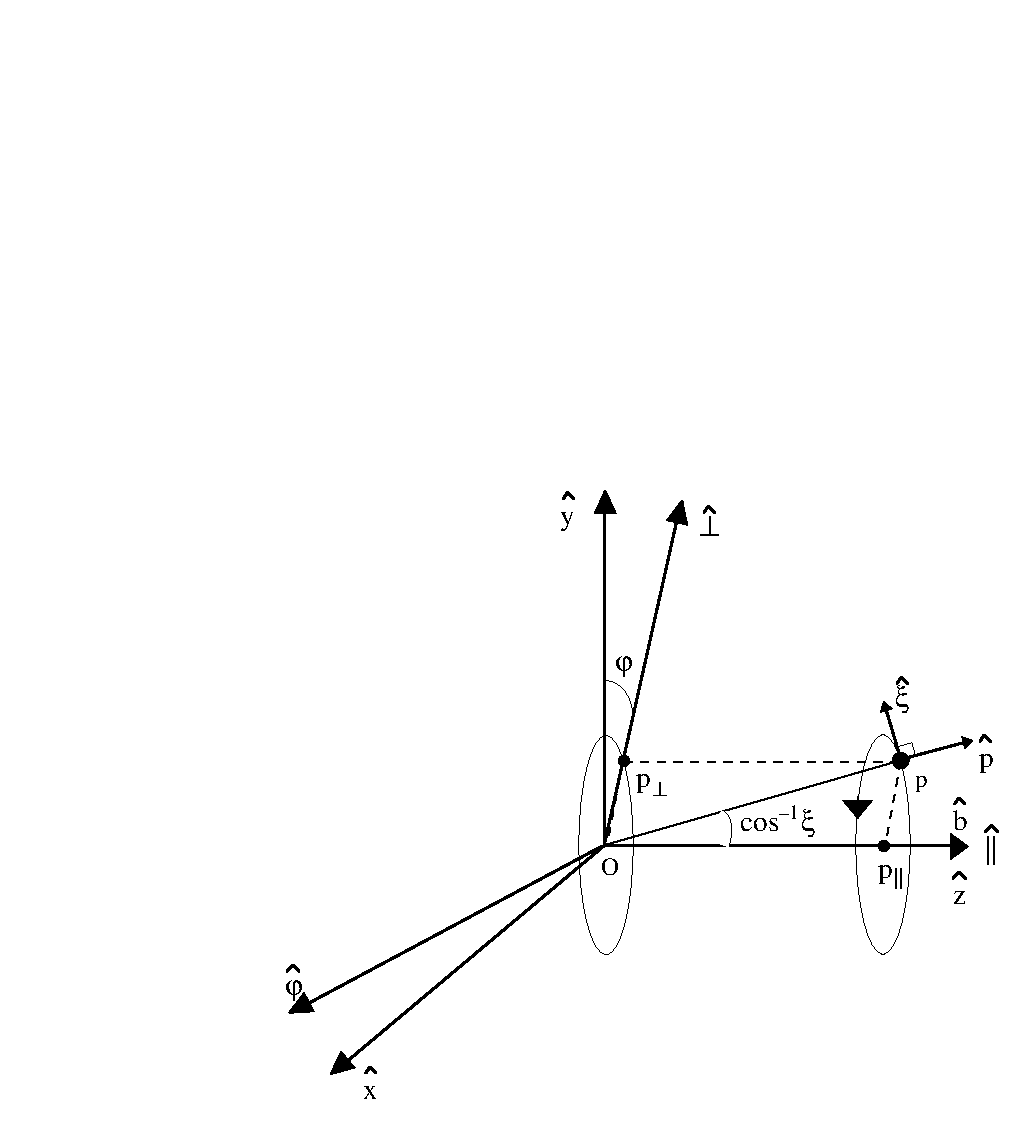
\includegraphics[width=3.6in]{figures/momentum.eps}
\end{center}
\caption{Momentum space coordinates systems $\left( p_{\Vert},p_{\bot },%
\protect\varphi\right) $ and $\left( p,\protect\xi,\protect\varphi\right) $.}
\label{figmomentum}
\end{figure}

The momentum space and the two systems are shown on Fig. \ref{figmomentum}.
In a relativistic plasma, the velocity is related to the momentum by (\ref%
{vdef0})%
\begin{equation}
\mathbf{v}=\dfrac{\mathbf{p}}{\gamma m_{e}}   \label{vdef}
\end{equation}
where (\ref{gammadef0})%
\begin{equation}
\gamma\left( \left\Vert \mathbf{p}\right\Vert \right) =\sqrt{1+\dfrac {%
p_{\Vert}^{2}+p_{\bot}^{2}}{m_{e}^{2}c^{2}}}=\sqrt{1+\dfrac{p^{2}}{%
m_{e}^{2}c^{2}}}   \label{gammadef}
\end{equation}
is the relativistic factor.

The motion of an electron in a uniform magnetic field is decomposed into a
gyration in the plane perpendicular to the field line and a free streaming
along the field line \cite{haz91b1}. The radius of the gyration, also called
electron Larmor radius or gyroradius, is 
\begin{equation}
\rho_{L}=\dfrac{p_{\bot}}{m_{e}\omega_{ce}}
\end{equation}
where 
\begin{equation}
\omega_{ce}=\dfrac{eB}{m_{e}}   \label{gyrorest}
\end{equation}
is the rest mass gyrofrequency. When the magnetic field is non-uniform and
when its variations, both in amplitude and directions, occur on a scale
length much larger than the Larmor radius, then the modifications to the
particle motion can be viewed as a perturbation to the gyromotion, and
consists of relatively slow particle drifts. When averaged over the fast
gyro-motion, the resulting velocity - called guiding center velocity - is
then the sum of the fast streaming along field lines and a slow drift%
\begin{equation}
\mathbf{v}_{\text{gc}}=v_{\Vert}\widehat{\mathbf{b}}+\mathbf{v}_{D} 
\label{vgc}
\end{equation}
where $\widehat{b}=\mathbf{B}/B$ is the unit vector in the magnetic field
direction.

In a constant equilibrium and the absence of equilibrium electric field, the
drift velocity $\mathbf{v}_{D}$ is the sum of the $\mathbf{\nabla}B$ drift,
due to changes in the magnitude of $\mathbf{B}$, and the curvature drift,
due to changes in the direction of $\mathbf{B}$. It is given by \cite%
{haz91b1}%
\begin{equation}
\mathbf{v}_{D}=\dfrac{1}{\Omega_{e}}\left( v_{\Vert}^{2}+\dfrac{v_{\bot}^{2}%
}{2}\right) \dfrac{\mathbf{B}\times\mathbf{\nabla}B}{B^{2}}   \label{vdrift0}
\end{equation}
where $\Omega_{e}$ is the relativistic cyclotron frequency%
\begin{equation}
\Omega_{e}=\dfrac{q_{e}B}{\gamma m_{e}}=-\dfrac{\omega_{ce}}{\gamma} 
\label{gyrofrequency}
\end{equation}

\subsection{Constants of the motion and particle motion along the field lines%
}

Because magnetic fields cannot do any work on charged particles, the
electron's kinetic energy $\mathcal{E}$ is a constant of the motion 
\begin{equation}
\dfrac{d\mathcal{E}}{dt}=0
\end{equation}
where $\mathcal{E}$ is expressed relativistically as%
\begin{equation}
\mathcal{E}=\left( \gamma-1\right) mc^{2}   \label{encons30}
\end{equation}

In addition, the fast gyromotion results in the existence of an adiabatic
invariant \cite{haz91b1}, 
\begin{equation}
\dfrac{d\mu}{dt}\simeq0   \label{mucons0}
\end{equation}
where $\mu$ is the magnetic moment%
\begin{equation}
\mu=\dfrac{p_{\bot}^{2}}{2\gamma m_{e}B}=\dfrac{q_{e}v_{\bot}^{2}}{2\Omega
_{e}}   \label{mu}
\end{equation}
Because of the conservation of energy and magnetic moment, the parallel
velocity of the electron decreases as it moves towards regions of higher
magnetic field amplitude. This effective force in the parallel direction is
called mirror force, as it is the principal longitudinal confining effect in
a mirror machine. In a toroidal plasma, the parallel velocity of an electron
moving towards higher field regions can sometimes vanish before the
electrons reaches the location of maximum magnetic field $B_{\max}\left(
\psi\right) $. In that case, the electron bounces back towards lower field
regions, and is called a trapped electron, as it is confined in a region of
low magnetic field. All electrons confined on a given flux surface $\psi$
will pass by the point of lowest magnetic field $B_{0}\left( \psi\right) $
on that flux-surface. In an axisymmetric plasma, it is therefore possible to
identify electrons by the value of their momentum components $p_{\Vert0}$
and $p_{\bot0}$ as they reach the point where $B\left( \psi,\theta\right)
=B_{0}\left( \psi\right) $.

The turning points $\theta_{T}$ in the bounce motion are then determined by
the location where $v_{\Vert}$ vanishes. The conservation of energy (\ref%
{encons30}) leads to the conservation of $\gamma$ and therefore, using (\ref%
{gammadef})%
\begin{equation}
p_{\Vert0}^{2}+p_{\bot0}^{2}=p_{\Vert}^{2}+p_{\bot}^{2}   \label{encons3}
\end{equation}
while the conservation of magnetic moment (\ref{mu}) gives%
\begin{equation}
\dfrac{p_{\bot0}^{2}}{B_{0}\left( \psi\right) }=\dfrac{p_{\bot}^{2}}{B\left(
\psi,\theta_{T}\right) }   \label{mucons}
\end{equation}
We define the ratio $\Psi\left( \psi,\theta\right) $, on a given flux
surface, between the magnetic field and its minimum value $B_{0}\left(
\psi\right) $ on that flux-surface.%
\begin{equation}
\Psi\left( \psi,\theta\right) \equiv\dfrac{B\left( \psi,\theta\right) }{%
B_{0}\left( \psi\right) }   \label{psidef}
\end{equation}
so that, at the turning point where $p_{\Vert}=0$, (\ref{mucons}) with (\ref%
{encons3}) gives 
\begin{equation}
\Psi\left( \psi,\theta_{T}\right) =1+\dfrac{p_{\Vert0}^{2}}{p_{\bot0}^{2}} 
\label{psithetaT}
\end{equation}
Trapped electrons are such that there exists such poloidal location $%
\theta_{T}$ and therefore%
\begin{equation}
1+\dfrac{p_{\Vert0}^{2}}{p_{\bot0}^{2}}<\Psi_{\max}\left( \psi\right)
\end{equation}
where $\Psi_{\max}\left( \psi\right) \equiv B_{\max}\left( \psi\right)
/B_{0}\left( \psi\right) $. The two turning points are 
\begin{equation}
\begin{array}{l}
\theta_{T\min}\left( p_{\Vert0},p_{\bot0},\psi\right) \equiv\min\left\{
\theta\left\vert B\left( \psi,\theta_{T}\right) \leq\left( 1+\dfrac {%
p_{\Vert0}^{2}}{p_{\bot0}^{2}}\right) B_{0}\left( \psi\right) \right.
\right\} \\ 
\\ 
\theta_{T\max}\left( p_{\Vert0},p_{\bot0},\psi\right) \equiv\max\left\{
\theta\left\vert B\left( \psi,\theta_{T}\right) \leq\left( 1+\dfrac {%
p_{\Vert0}^{2}}{p_{\bot0}^{2}}\right) B_{0}\left( \psi\right) \right.
\right\}%
\end{array}
\label{thetaT}
\end{equation}
and we have $\theta_{T\min}=-\theta_{T\max}$ in an up-down symmetric plasma.

In spherical momentum coordinates $\left( p,\xi\right) $, the conservation
of energy (\ref{encons30}) gives 
\begin{equation}
p_{0}=p
\end{equation}
meaning that the magnitude of the particle momentum is conserved, while the
conservation of magnetic moment (\ref{mucons}) leads to%
\begin{equation}
\dfrac{1-\xi_{0}^{2}}{B_{0}\left( \psi\right) }=\dfrac{1-\xi^{2}}{B\left(
\psi,\theta\right) }   \label{mucons2}
\end{equation}
so that, at the turning point where $\xi=0$,%
\begin{equation}
\Psi\left( \psi,\theta_{T}\right) =\dfrac{1}{1-\xi_{0}^{2}}   \label{Psidef}
\end{equation}
Trapped electrons on a given flux-surface are therefore such that%
\begin{equation}
\xi_{0}^{2}<\xi_{0T}^{2}\left( \psi\right)
\end{equation}
where we defined%
\begin{equation}
\xi_{0T}\left( \psi\right) \equiv\sqrt{1-\dfrac{1}{\Psi_{\max}\left(
\psi\right) }}   \label{xi0t2}
\end{equation}

In spherical coordinates, electrons are therefore identified by their
momentum $p$, which is a constant of the motion, and by the value $\xi_{0}$
of their pitch-angle as they cross the point of minimum $B$-field on the
flux-surface. The turning points (\ref{thetaT}) of an electron ($p,\xi_{0}$)
can also be defined in $\left( p,\xi\right) $ coordinates, using (\ref%
{Psidef})%
\begin{equation}
\begin{array}{l}
\theta_{T\min}\left( \xi_{0},\psi\right) \equiv\min\left\{ \theta\left\vert
B\left( \psi,\theta_{T}\right) \leq\dfrac{B_{0}\left( \psi\right) }{%
1-\xi_{0}^{2}}\right. \right\} \\ 
\\ 
\theta_{T\max}\left( \xi_{0},\psi\right) \equiv\max\left\{ \theta\left\vert
B\left( \psi,\theta_{T}\right) \leq\dfrac{B_{0}\left( \psi\right) }{%
1-\xi_{0}^{2}}\right. \right\}%
\end{array}
\label{thetaT2}
\end{equation}
The pitch-angle of an electron varies along the flux-surface according to (%
\ref{mucons2})%
\begin{equation}
\xi=\sigma\sqrt{1-\Psi\left( \psi,\theta\right) \left( 1-\xi_{0}^{2}\right) }
\label{xi}
\end{equation}
where $\sigma=$sign$(\xi_{0})$. We can also derive the condition for an
electron with pitch-angle $\xi$ at the poloidal location $\theta$ to be
trapped. From (\ref{mucons2}) and (\ref{xi0t2}) the condition is%
\begin{equation}
\xi<\xi_{T}\left( \psi,\theta\right) =\sqrt{1-\dfrac{\Psi\left( \psi
,\theta\right) }{\Psi_{\max}\left( \psi\right) }}
\end{equation}
We define the limits $\theta_{\min}$ and $\theta_{\max}$ as 
\begin{equation}
\begin{array}{c}
\theta_{\min}\left( \psi,\xi_{0}\right) =\left\{ 
\begin{array}{cc}
-\pi & \text{for passing particles} \\ 
\theta_{T\min} & \text{for trapped particles}%
\end{array}
\right. \\ 
\theta_{\max}\left( \psi,\xi_{0}\right) =\left\{ 
\begin{array}{cc}
\pi & \text{for passing particles} \\ 
\theta_{T\max} & \text{for trapped particles}%
\end{array}
\right.%
\end{array}
\label{thetaT3}
\end{equation}
where $\theta_{T\min}$ and $\theta_{T\max}$ were defined in (\ref{thetaT2}).
The conditions for an electron ($p,\xi_{0}$) to be able to reach a given
poloidal location $\theta$ is then 
\begin{equation}
\theta_{\min}\left( \psi,\xi_{0}\right) \leq\theta\leq\theta_{\max}\left(
\psi,\xi_{0}\right)   \label{thetacond}
\end{equation}
which, using (\ref{psithetaT}), can also be written as%
\begin{equation}
\Psi\left( \psi,\theta\right) \leq\dfrac{1}{1-\xi_{0}^{2}}
\end{equation}
or equivalently%
\begin{equation}
\left\vert \xi_{0}\right\vert \geq\sqrt{1-\dfrac{1}{\Psi\left( \psi
,\theta\right) }}   \label{xi0cond}
\end{equation}

\subsection{Particle drift in an axisymmetric toroidal plasma}

In an axisymmetric toroidal plasma, the equilibrium magnetic field is given
by (\ref{B}), which is rewritten in $\left( \psi,s,\phi\right) $ coordinates
as 
\begin{equation}
\mathbf{B}=\frac{I\left( \psi\right) }{R}\widehat{\phi}+\dfrac{\left\Vert 
\mathbf{\nabla}\psi\right\Vert }{R}\widehat{s}   \label{bexp2}
\end{equation}
and is necessarily non-uniform. In that case, particles are subject to
drifts both within and across the flux-surfaces. We are particularly
interested in drifts across the flux-surfaces as they are essentially
responsible for the existence of the bootstrap current.

\subsubsection{Drift Velocity from the Expression of Single Particle Drift}

The guiding-center drift velocity due to the magnetic field gradient and
curvature is given by (\ref{vdrift0}) and its component perpendicular to the
flux-surface can be written as 
\begin{equation}
\mathbf{v}_{D}\cdot\mathbf{\nabla}\psi=\frac{1}{\Omega_{e}}\left( v_{\Vert
}^{2}+\frac{v_{\bot}^{2}}{2}\right) \frac{1}{B^{2}}\mathbf{\nabla}\psi \times%
\mathbf{B}\cdot\mathbf{\nabla}B
\end{equation}
Inserting the expression (\ref{bexp2}) of the magnetic field, we find 
\begin{equation}
\mathbf{v}_{D}\cdot\nabla\psi=\frac{1}{\Omega_{e}}\left( v_{\Vert}^{2}+\frac{%
v_{\bot}^{2}}{2}\right) \frac{\left\Vert \mathbf{\nabla}\psi\right\Vert }{%
B^{2}R}\left[ \left\Vert \mathbf{\nabla}\psi\right\Vert \widehat{\phi}%
-I\left( \psi\right) \widehat{s}\right] \cdot\mathbf{\nabla}B   \label{drift}
\end{equation}
Using axisymmetry and the expression (\ref{gradpsisphi}) for the gradient in 
$\left( \psi,s,\phi\right) $ coordinates, the equation (\ref{drift}) becomes 
\begin{equation}
\mathbf{v}_{D}\cdot\nabla\psi=-\frac{1}{\Omega_{e}}\left( v_{\Vert}^{2}+%
\frac{v_{\bot}^{2}}{2}\right) \frac{\left\Vert \mathbf{\nabla}%
\psi\right\Vert I\left( \psi\right) }{B^{2}R}\frac{\partial B}{\partial s}
\end{equation}
With the definition (\ref{mu}) of the magnetic moment $\mu$, we rewrite 
\begin{equation}
\mathbf{v}_{D}\cdot\nabla\psi=-\frac{1}{\Omega_{e}}\frac{\left\Vert \mathbf{%
\nabla}\psi\right\Vert I\left( \psi\right) }{B^{2}R}\left( v_{\Vert}^{2}+%
\dfrac{\mu\Omega_{e}}{q_{e}}\right) \frac{\partial B}{\partial s} 
\label{drift2}
\end{equation}
Using the conservation of magnetic moment (\ref{mucons0}) along the particle
motion 
\begin{equation}
\dfrac{\mu\Omega_{e}}{q_{e}}\frac{\partial B}{\partial s}=\Omega_{e}\frac{%
\partial}{\partial s}\left( \frac{\mu B}{q_{e}}\right)
\end{equation}
and using the conservation of energy (\ref{encons30}) and the identity%
\begin{equation}
\dfrac{v_{\Vert}^{2}}{B}\frac{\partial B}{\partial s}=\frac{\partial}{%
\partial s}\left( \dfrac{v_{\Vert}^{2}}{2}\right) -v_{\Vert}B\frac{\partial}{%
\partial s}\left( \dfrac{v_{\Vert}}{B}\right)
\end{equation}
we get%
\begin{equation}
\dfrac{1}{B}\left( v_{\Vert}^{2}+\dfrac{\mu\Omega_{e}}{q_{e}}\right) \frac{%
\partial B}{\partial s}=-v_{\Vert}B\frac{\partial}{\partial s}\left( \dfrac{%
v_{\Vert}}{B}\right)
\end{equation}
and finally, the equation (\ref{drift2}) becomes 
\begin{equation}
\mathbf{v}_{D}\cdot\mathbf{\nabla}\psi=\frac{v_{\Vert}}{\Omega_{e}}I\left(
\psi\right) \frac{\left\Vert \mathbf{\nabla}\psi\right\Vert }{R}\frac{%
\partial}{\partial s}\left( \frac{v_{\Vert}}{B}\right)   \label{drift3}
\end{equation}
In addition, using (\ref{bexp2}) and axisymmetry, 
\begin{equation}
\mathbf{B}\cdot\mathbf{\nabla}=\frac{\left\Vert \mathbf{\nabla}%
\psi\right\Vert }{R}\frac{\partial}{\partial s}   \label{bdotgrad}
\end{equation}
so that we can rewrite (\ref{drift3}) as 
\begin{equation}
\mathbf{v}_{D}\cdot\mathbf{\nabla}\psi=\frac{v_{\Vert}}{\Omega_{e}}I\left(
\psi\right) \mathbf{B}\cdot\mathbf{\nabla}\left( \frac{v_{\Vert}}{B}\right) 
\label{vdpsi2}
\end{equation}

\subsubsection{Drift velocity from the conservation of canonical momentum}

The drift velocity (\ref{vdpsi2}) was obtained based on the expression (\ref%
{vdrift0}), which was not derived from first principles. Note that we can
also derive the drift velocity using the conservation of canonical momentum,
which is also a constant of the motion because of axisymmetry. It is
expressed as 
\begin{equation}
P_{\phi}=R\left[ \gamma m_{e}v_{\phi}+q_{e}A_{\phi}\right]
\end{equation}
where $A_{\phi}$ is the toroidal component of the vector potential.

From the relation 
\begin{equation}
\mathbf{B}=\nabla\times\mathbf{A}
\end{equation}
with the expression (\ref{curlpsisphi}) of a curl in $\left( \psi
,s,\phi\right) $ coordinates, we have 
\begin{equation}
B_{s}=\dfrac{1}{R}\dfrac{\partial}{\partial\phi}\left( A_{\psi}\right) -%
\dfrac{\left\Vert \mathbf{\nabla}\psi\right\Vert }{R}\dfrac{\partial }{%
\partial\psi}\left( RA_{\phi}\right)
\end{equation}
Then, using axisymmetry and the expression (\ref{Bp1}) for the poloidal
field, we get 
\begin{equation}
RA_{\phi}=-\psi   \label{aphipsi}
\end{equation}
where we chose arbitrarily $A_{\phi}\left( \psi=0\right) =0$.

Because the toroidal canonical momentum is a constant of the motion, we have
\thinspace%
\begin{equation}
\mathbf{v}_{\text{gc}}\cdot\nabla P_{\phi}=0
\end{equation}
which becomes, using (\ref{vgc}), (\ref{aphipsi}) and the conservation of
energy so that $\mathbf{v}_{\text{gc}}\cdot\nabla\gamma=0$, 
\begin{equation}
\mathbf{v}_{D}\cdot\nabla\psi=\dfrac{\gamma m_{e}}{q_{e}}\mathbf{v}_{\text{gc%
}}\cdot\nabla\left( Rv_{\phi}\right)   \label{eqpphi}
\end{equation}
Assuming a priori that $\left\vert v_{\Vert}\right\vert \gg\left\vert 
\mathbf{v}_{D}\right\vert $, a condition that is well verified consistent
with the conservation of magnetic moment, this equation reduces to 
\begin{equation}
\mathbf{v}_{D}\cdot\nabla\psi=\dfrac{\gamma m_{e}}{q_{e}B}v_{\Vert}\mathbf{B}%
\cdot\nabla\left( Rv_{\phi}\right) =\frac{v_{\Vert}}{\Omega_{e}}\mathbf{B}%
\cdot\nabla\left( Rv_{\phi}\right)
\end{equation}
The toroidal velocity is related to the parallel velocity by 
\begin{equation}
v_{\phi}=\frac{B_{\phi}}{B}v_{\Vert}=\frac{I\left( \psi\right) }{RB}v_{\Vert}
\end{equation}
Since $I\left( \psi\right) $ is a flux function, it can be taken out of the
gradient, so that 
\begin{equation}
\mathbf{v}_{D}\cdot\nabla\psi=\frac{v_{\Vert}}{\Omega_{e}}I\left(
\psi\right) \mathbf{B}\cdot\nabla\left( \frac{v_{\Vert}}{B}\right) 
\label{vdpsi1}
\end{equation}
an expression which is the same as (\ref{vdpsi2}).

\subsubsection{Deviation of particle orbits from the flux-surface}

\begin{figure}[tbh]
\begin{center}
\includegraphics[width=3.6in]{figures/banana.eps}
\end{center}
\caption{Poloidal projection of particle orbits in a toroidal plasma.}
\label{drifts}
\end{figure}

Because of the drift across flux-surfaces, particles are not strictly
confined to a given flux-surface. Considering that the gradient of magnetic
field amplitude is globally in the inward direction ($\mathbf{\nabla}B\simeq
-\widehat{\mathbf{R}}B/R$), the drift velocity in the poloidal plane (\ref%
{vdrift0}) is arroximately%
\begin{equation}
v_{DP}\simeq-\dfrac{1}{\Omega_{e}}\left( v_{\Vert}^{2}+\dfrac{v_{\bot}^{2}}{2%
}\right) \dfrac{B_{T}}{RB}\widehat{\mathbf{Z}}   \label{vdp}
\end{equation}
and is therefore directed in the vertical direction. Because ions and
electrons drift in opposite direction, this drift could generate a vertical
electric field that would lead to a loss of confinement due to resulting $%
\mathbf{E}\times\mathbf{B}$ drift in the outboard direction. However, along
the poloidal motion of particles, this drift is directed alternatively
towards the core and toward the edge of the plasma, such that it cancels
exactly over the course of one transit or bounce period. This explains why a
poloidal field is necessary to confine a ST or tokamak plasma. Although the
cumulative drift vanishes over one poloidal motion, particles drift across
the flux-surfaces along their orbit, as illustrated on figure \ref{drifts},
which results of the characteristic shape for trapped electrons, called 
\textit{banana orbits}. The maximum deviation off the flux-surface can be
estimated by calculating the accumulated drift over half a bounce or transit
time $\tau_{b}$. From (\ref{vdp}), we get%
\begin{equation}
\Delta r_{D}\simeq v_{DP}\dfrac{\tau_{b}}{2}\simeq\left\{ 
\begin{array}{ll}
\rho_{Te}\pi q & \text{for passing electrons} \\ 
&  \\ 
\rho_{Te}\dfrac{\pi q}{\xi_{0T}} & \text{for trapped electrons}%
\end{array}
\right.   \label{drd}
\end{equation}
where we used the estimation (\ref{taubest}) for the bounce time and where
we used $q\simeq\widetilde{q}B_{T}/B$. We see that the particle deviation
from the flux-surface is not more than a few Larmor radii, and that it is
larger for trapped electrons, because their parallel velocity is smaller.

\subsection{Bounce time and bounce averaging operation}

\subsubsection{Transit or Bounce Time\label{bavsec}}

\bigskip Because the orbit deviation from a flux-surface is very small
compared to the size of the plasma and the poloidal orbit length, it is a
good approximation, for electrons, to assume that the particle is exactly on
the flux-surface when integrating along the particle orbit. In this limit of
zero-banana width, the forward and backward motion of trapped electrons
follow the same trajectory. In that case, we can define the bounce time as
the time for a trapped electron to complete half a bounce period. The
poloidal transit time for a passing electron is defined as the time to
complete a full orbit in the poloidal plane. We define then, for any
electron 
\begin{equation}
\tau_{b}\left( \psi\right) =\int_{s_{\min}}^{s_{\max}}\frac{ds}{\left\vert
v_{s}\right\vert }=\int_{s_{\min}}^{s_{\max}}\frac{ds}{\left\vert v_{\Vert
}\right\vert }\frac{B}{B_{P}}   \label{taub}
\end{equation}
where $v_{s}$ is the guiding center velocity along the poloidal field lines,
and $v_{\Vert}$ is its velocity parallel to the magnetic field. The limits $%
s_{\min}$ and $s_{\max}$ are defined in (\ref{bmax}) for passing electrons,
and are the positions, along the field lines, of turning points for trapped
electrons.

%\fig{figures/vpar.eps}{Guiding center velocity definition}{figvpar}{7cm}

The differential arc length $ds$ along the poloidal field line is generally
expressed in curvilinear coordinates $\left( u^{1},u^{2},u^{3}\right) $ as (%
\ref{dl}) 
\begin{equation}
ds=\sqrt{g_{ij}du^{i}du^{j}}   \label{dl2}
\end{equation}
where the $g_{ij}$ are the metric coefficients, defined in (\ref{met}). In
the $\left( \psi,\theta,\phi\right) $ coordinates system, the variations $%
d\psi$ and $d\phi$ are essentially zero along the poloidal field line. As a
consequence, (\ref{dl2}) reduces to 
\begin{equation}
ds=\sqrt{g_{22}}d\theta   \label{dsdtheta}
\end{equation}
where the metric factor $\sqrt{g_{22}}$ represent the poloidal distance per
radian along the field lines. The bounce time (\ref{taub}) becomes%
\begin{equation}
\tau_{b}\left( \psi\right) =\int_{\theta_{\min}}^{\theta_{\max}}d\theta 
\frac{\sqrt{g_{22}}}{\left\vert v_{\Vert}\right\vert }\frac{B}{B_{P}}
\end{equation}
where the limits$\ \theta_{\min}$ and $\theta_{\max}$ are defined in (\ref%
{thetaT3}).

In spherical momentum coordinates, we have (\ref{pxidef})%
\begin{equation}
\frac{v_{\Vert}}{v}=\frac{p_{\Vert}}{p}=\xi
\end{equation}
so that 
\begin{equation}
\tau_{b}\left( \psi\right) =\frac{2\pi}{v\left\vert \xi_{0}\right\vert }%
\int_{\theta_{\min}}^{\theta_{\max}}\frac{d\theta}{2\pi}\sqrt{g_{22}}\frac {%
\xi_{0}}{\xi}\frac{B}{B_{P}}
\end{equation}

The bounce time can then be normalized as 
\begin{equation}
\tau_{b}\left( \psi,\xi_{0}\right) =\frac{2\pi R_{p}\widetilde{q}\left(
\psi\right) }{v\left\vert \xi_{0}\right\vert }\lambda\left( \psi,\xi
_{0}\right)   \label{Normbtime}
\end{equation}
where 
\begin{equation}
\lambda\left( \psi,\xi_{0}\right) =\frac{1}{\widetilde{q}\left( \psi\right) }%
\int_{\theta_{\min}}^{\theta_{\max}}\frac{d\theta}{2\pi}\frac{\sqrt{g_{22}}}{%
R_{p}}\frac{\xi_{0}}{\xi}\frac{B}{B_{P}}   \label{lambda0}
\end{equation}
and 
\begin{equation}
\widetilde{q}\left( \psi\right) \equiv\int_{0}^{2\pi}\frac{d\theta}{2\pi }%
\frac{\sqrt{g_{22}}}{R_{p}}\frac{B}{B_{P}}
\end{equation}
The bounce time is in fact normalized to the transit time of particles with
parallel momentum only, since $\lambda\left( \psi,\pm1\right) =1$. The
factor $\widetilde{q}\left( \psi\right) $ represents the length of field
lines within one poloidal rotation, normalized by $2\pi R_{p}$.

The covariant metric element $g_{22}$ is given by (\ref{rel1})-(\ref{met}),
which in the $\left( \psi,\theta,\phi\right) $ system becomes (\ref%
{covpsithetaphi}) 
\begin{equation}
g_{22}=\frac{r}{\left\vert \widehat{\mathbf{\psi}}\cdot\widehat{\mathbf{r}}%
\right\vert }   \label{g22}
\end{equation}

Consequently, the normalized bounce time takes the form 
\begin{equation}
\lambda\left( \psi,\xi_{0}\right) =\frac{1}{\widetilde{q}\left( \psi\right) }%
\int_{\theta_{\min}}^{\theta_{\max}}\frac{d\theta}{2\pi}\frac {1}{\left\vert 
\widehat{\mathbf{\psi}}\cdot\widehat{\mathbf{r}}\right\vert }\frac{r}{R_{p}}%
\frac{B}{B_{P}}\frac{\xi_{0}}{\xi}   \label{lambda}
\end{equation}
with 
\begin{equation}
\widetilde{q}\left( \psi\right) =\int_{0}^{2\pi}\frac{d\theta}{2\pi}\frac {1%
}{\left\vert \widehat{\psi}\cdot\widehat{r}\right\vert }\frac{r}{R_{p}}\frac{%
B}{B_{P}}   \label{qtilde}
\end{equation}

\subsubsection{Bounce Averaging}

Anticipating that the kinetic equation will be reduced based on the fast
streaming motion along the field lines, we define an average over the
poloidal motion, which accounts for changes in the particle velocity,
including trapping, and effectively annihilates any term of the type $%
\mathbf{v}_{s}\cdot\partial/\partial s$ in the zero banana-width limit. This
is called the bounce-averaging operation 
\begin{align}
\left\{ \mathcal{A}\right\} & =\frac{1}{\tau_{b}}\left[ \frac{1}{2}%
\sum_{\sigma}\right] _{T}\int_{s_{\min}}^{s_{\max}}\frac{ds}{\left\vert
v_{s}\right\vert }\mathcal{A}  \notag \\
& =\frac{1}{\tau_{b}}\left[ \frac{1}{2}\sum_{\sigma}\right]
_{T}\int_{s_{\min}}^{s_{\max}}\frac{ds}{\left\vert v_{\Vert}\right\vert }%
\frac {B}{B_{P}}\mathcal{A}   \label{bav02}
\end{align}
where the sum over $\sigma=$sign$\left( v_{\Vert}\right) $ applies to
trapped particles only. This is an average over a poloidal rotation for
passing electrons, and over both the forward and backward motion for trapped
electrons. It can be rewritten in $\left( \psi,\theta,\phi\right) $
coordinates using (\ref{dsdtheta})%
\begin{equation}
\left\{ \mathcal{A}\right\} =\frac{1}{\tau_{b}}\left[ \frac{1}{2}%
\sum_{\sigma}\right] _{T}\int_{\theta_{\min}}^{\theta_{\max}}d\theta \frac{%
\sqrt{g_{22}}}{\left\vert v_{\Vert}\right\vert }\frac{B}{B_{P}}\mathcal{A}
\end{equation}
and in terms of the normalized bounce time $\lambda$ using expression (\ref%
{lambda0}) 
\begin{equation}
\left\{ \mathcal{A}\right\} =\frac{1}{\lambda\widetilde{q}}\left[ \frac {1}{2%
}\sum_{\sigma}\right] _{T}\int_{\theta_{\min}}^{\theta_{\max}}\frac{d\theta}{%
2\pi}\frac{\sqrt{g_{22}}}{R_{p}}\frac{B}{B_{P}}\frac{\xi_{0}}{\xi}\mathcal{A}
\label{bav}
\end{equation}
or, inserting the expression (\ref{g22}) for $\sqrt{g_{22}}$ 
\begin{equation}
\left\{ \mathcal{A}\right\} =\frac{1}{\lambda\widetilde{q}}\left[ \frac {1}{2%
}\sum_{\sigma}\right] _{T}\int_{\theta_{\min}}^{\theta_{\max}}\frac{d\theta}{%
2\pi}\frac{1}{\left\vert \widehat{\psi}\cdot\widehat {\mathbf{r}}\right\vert 
}\frac{r}{R_{p}}\frac{B}{B_{P}}\frac{\xi_{0}}{\xi }\mathcal{A}   \label{bav2}
\end{equation}

We anticipate that bounce averaging the momentum-space operators in the
kinetic equations leads to a set of coefficients that all have a similar
structure, denoted $\lambda_{k,l,m}$ and $\overline{\lambda}_{k,l,m}$, which
are define as 
\begin{equation}
\left\{ \left( \frac{\xi\left( \psi,\theta,\xi_{0}\right) }{\xi_{0}}\right)
^{k}\Psi^{l}\left( \psi,\theta\right) \left( \frac{R_{0}\left( \psi\right) }{%
R\left( \psi,\theta\right) }\right) ^{m}\right\} \equiv\frac{%
\lambda_{k,l,m}\left( \psi,\xi_{0}\right) }{\lambda\left(
\psi,\xi_{0}\right) }   \label{lkm}
\end{equation}
and 
\begin{equation}
\sigma\left\{ \sigma\left( \frac{\xi\left( \psi,\theta,\xi_{0}\right) }{%
\xi_{0}}\right) ^{k}\Psi^{l}\left( \psi,\theta\right) \left( \frac {%
R_{0}\left( \psi\right) }{R\left( \psi,\theta\right) }\right) ^{m}\right\}
\equiv\frac{\overline{\lambda}_{k,l,m}\left( \psi,\xi _{0}\right) }{%
\lambda\left( \psi,\xi_{0}\right) }   \label{lkmb}
\end{equation}
where 
\begin{equation}
R_{0}\left( \psi\right) \equiv R\left( \psi,\theta_{0}\right)
\end{equation}

Note that by definition, $\lambda_{0,0,0}=\lambda$. In addition, 
\begin{equation}
\overline{\lambda}_{k,l,m}=\left\vert 
\begin{array}{ll}
\lambda_{k,l,m} & \text{ for passing particles} \\ 
0 & \text{ for trapped particles}%
\end{array}
\right.
\end{equation}
